\documentclass[a4paper, 11pt]{article}

\usepackage{geometry}
%\geometry{a4paper,left=30mm,right=30mm, top=20mm, bottom=20mm}
\geometry{a4paper,left=20mm,right=20mm, top=25mm, bottom=20mm}

\usepackage[ngerman]{babel}
\usepackage[utf8]{inputenc} 
\usepackage[T1]{fontenc}
\usepackage{amsmath}
\usepackage{amssymb}
\usepackage{fancyhdr}
\usepackage{graphicx}
\usepackage{tikz}
\usepackage{lscape}
\usepackage{comment}
\usetikzlibrary{positioning}

\usepackage{lastpage} % Seitenzahlen

\pagestyle{fancy}
\usepackage{mathtools}   % Lädt »amsmath« 
\newtagform{simple}{}{}{}
\usetagform{simple}

\usepackage{tabularx} %schöne tabellen
\parindent0pt %einrücken verhindern

\usepackage{polynom}
% overall sans serif font
%\renewcommand{\familydefault}{\sfdefault}
\cfoot{\thepage  \ / \pageref{LastPage}}

% % % % % % % % % % % % % % % % % % % % % % % %
% % % % % % % % % % % % % % % % % % % % % % % %
\newcommand{\modullang}{AOT}
\newcommand{\modul}{AOT MSC}
\newcommand{\blatt}{02 Übungsblatt}
\newcommand{\tutorium}{Mittwoch 12:00 Uhr}
\newcommand{\tutor}{Dr. Fricke}
\newcommand{\datum}{21. Dezember 2014}
\newcommand{\gruppe}{Gr02}
\newcommand{\RM}[1]{\MakeUppercase{\romannumeral #1}}
% % % % % % % % % % % % % % % % % % % % % % % %
% % % % % % % % % % % % % % % % % % % % % % % %

\begin{document} 

%%% Kopfzeile linker Bereich
%      gerade Seite   ungerade Seite
\lhead{\textbf{\modul}}
%%% Kopfzeile mittlerer Bereich
%      gerade Seite   ungerade Seite
%\chead{\blatt}
%%% Kopfzeile linker Bereich
%      gerade Seite             ungerade Seite
\rhead{\gruppe}


	%-- Deckblatt --						      
	\title{\textbf{\modullang\\[0.25cm]}
		\normalsize{\blatt}} %Thema ändern	
	\author{\tutorium\\ \\
		Mitja Richter, 324680\\
		Tobias Pockrandt, 325550\\
		Seitenzahl: \pageref{LastPage} \\ \\ \\ \\
		%Professor: Knipping\\
		Tutor: \tutor}
	\date{Abgabedatum: \datum} %Datum ändern
	\maketitle
	\newpage
	
	%\renewcommand \thesection {\arabic{section}.}
	%\renewcommand \thesubsection {\thesection. \arabic{subsection}}
	%\renewcommand \thesubsubsection {\thesubsection. \arabic{subsubsection}}
	

\renewcommand{\labelenumi}{\alph{enumi})}
\renewcommand{\labelenumii}{(\roman{enumii})}
\renewcommand{\labelenumiii}{\arabic{enumiii}.}
%\renewcommand{\labelenumii}{\textbf{-}}	
%-- Eigentlicher Text --
\section*{1. Aufgabe - Schulze Methode\hfill {\small (5 Punkte)}}
\begin{enumerate}
\item
\begin{tabular}{c || c|c|c|c}
& zu A & zu B & zu C & zu D \\ \hline
A & & A-(15)-D-\underline{(11)}-C-(13)-B & A-(15)-D-\underline{(11)}-C & A-\underline{(15)}-D \\
B & B-\underline{(5)}-A & & B-(21)-D-\underline{(11)}-C  & B-\underline{(21)}-D \\
C & C-(13)-B-\underline{(5)}-A & C-\underline{(13)}-B & & C-\underline{(13)}-B-(21)-D \\
D & D-(17)-E-(9)-B-\underline{(5)}-A & D-\underline{(11)}-C-(13)-B & D-\underline{(11)}-C & \\
E & E-(9)-B-\underline{(5)}-A & E-\underline{(9)}-B & E-\underline{(9)}-B-(21)-D-(11)-C & E-\underline{(9)}-B-(21)


\end{tabular}\\
\begin{tabular}{c || c}
& zu E\\ \hline
A & A-\underline{(15)}-D-(17)-E\\
B  & B-(21)-D-\underline{(17)}-E\\
C & C-\underline{(13)}-B-(21)-D-(17)-E\\
D & D-\underline{(17)}-E\\
E &


\end{tabular}

\item 
\begin{align*}
p(A,B) > P(B,A) \rightarrow A \text{ besser als } B \\
p(A,C) > P(C,A) \rightarrow A \text{ besser als } C \\
p(A,D) > P(D,A) \rightarrow A \text{ besser als } D \\
p(A,E) > P(E,A) \rightarrow A \text{ besser als } E \\
\\
p(C,B) > P(B,C) \rightarrow C \text{ besser als } B \\
p(C,D) > P(D,C) \rightarrow C \text{ besser als } D \\
p(C,E) > P(E,C) \rightarrow C \text{ besser als } E \\
\\
p(B,D) > P(D,B) \rightarrow B \text{ besser als } D \\
p(B,E) > P(E,B) \rightarrow B \text{ besser als } E \\
\\
p(D,E) > P(E,D) \rightarrow D \text{ besser als } E \\
\\
\rightarrow A > C > B > D > E
\end{align*}
\end{enumerate}
\section*{2. Aufgabe - Machtverteilung im Weighted Voting\hfill {\small (5 Punkte)}}
\begin{enumerate}

\item 
$[100: 70, 60, 30, 10]$\\
- ungleiches Gewicht und Macht. Keine Diktatoren, Veto- oder Dummyspieler. Gewinnerkoalitionen:\\
$\{(P_1,P_2), (P_1,P_3), (P_1,P_2,P_3), (P_1,P_2,P_4), (P_1,P_3,P_4), (P_2,P_3,P_4), (P_1,P_2,P_3,P_4)\}$\\\\
\begin{tabular}{c | c | c}
  &  BPI & SSP\\ \hline
  $P_1$ & $6/7$ & $1/2$ \\ \hline
  $P_2$ & $3/7$ & $5/24$ \\ \hline
  $P_3$ & $3/7$ & $5/24$ \\ \hline
  $P_4$ & $1/7$ & $1/12$ \\ \hline
\end{tabular}

\item$[100: 110, 90, 5]$\\
- ungleiches Gewicht und Macht. $P_1$ ist Diktator, der Rest Dummyspieler. Gewinnerkoalitionen:\\
$\{(P_1), (P_1,P_2), (P_1,P_3), (P_1,P_2,P_3)\}$\\\\
\begin{tabular}{c | c | c}
  &  BPI & SSP\\ \hline
  $P_1$ & $1$ & $1$ \\ \hline
  $P_2$ & $0$ & $0$ \\ \hline
  $P_3$ & $0$ & $0$ \\ \hline
  $P_4$ & $0$ & $0$ \\ \hline
\end{tabular}


\item
$[100: 60, 40, 30, 20]$\\
- ungleiches Gewicht und Macht. $P_1$ ist Vetospieler. Gewinnerkoalitionen:\\
$\{(P_1,P_2), (P_1,P_2,P_3), (P_1,P_2,P_4), (P_1,P_3,P_4), (P_1,P_2,P_3,P_4)\}$\\\\
\begin{tabular}{c | c | c}
  &  BPI & SSP\\ \hline
  $P_1$ & $1$ & $3/4$ \\ \hline
  $P_2$ & $3/5$ & $1/6$ \\ \hline
  $P_3$ & $1/5$ & $1/24$ \\ \hline
  $P_4$ & $1/5$ & $1/24$ \\ \hline
\end{tabular}

\end{enumerate}
\section*{3. Aufgabe - Happy Hour in der Cocktailbar\hfill {\small (5 Punkte)}}
\begin{enumerate}
\item
Die einzige Imputation im Core wäre $(0,0,1)$ - d.h. $F$ kriegt alles und $M_1$ sowie $M_2$ nichts.
\item 
$(0.1,0.1,0.8)$ kann nicht im Core liegen, da hier $F$ mit einem der beiden $M$ ausscheren kann, um den kompletten Drink unter sich aufzuteilen - z.B. $M_1 = 0$, $M_2 =0.11$ und $F=0.89$.
\item
\begin{tabular}{c || c c c}
& $M_1$ & $M_2$ & $f$ \\ \hline
$M_1M_2F$ & 0 & 0 & 1 \\
$M_1FM_2 $ & 0 & 0 & 1 \\
$M_2M_1F$ & 0 & 0 & 1 \\
$M_2FM_1$ & 0 & 0 & 1 \\
$FM_1M_2$ & 1 & 0 & 0 \\
$FM_2M_1$ & 0 & 1 & 0 \\
SP & $\frac{1}{6}$ & $\frac{1}{6}$ & $\frac{4}{6}$ \\
\end{tabular}
\item
Für den Core gilt immer das Geschlecht, das weniger vorhanden ist, wird jeweils das komplette Getränk für sich haben können, da in jeder Situation mindestens zwei von der Gegenpartei um die Teilnahme in der 2er Koalition buhlen. Ist diese entschieden bleibt einer übrig der wiederum um eine andere Koalition buhlen muss und das Vorgehen wiederholt sich. Das bedeutet für 4M und 5F, dass alle M das Getränk bekommen und alle F nichts. Für 99M, 1F bedeutet es, dass F ein Getränk haben wird und der Rest nichts.\\

Bei dem Shapley-Value für 99M, 1F gibt es $100!$ mögliche Auszahlungsreihenfolgen. F kriegt nur keine Auszahlung, wenn Sie die erste in der Permutation ist, also in $99!$ Fällen. Das bedeutet, dass der SP für $F = 1 - \frac{99!}{100!} = \frac{99}{100}$ und da die M gleiches Gewicht besitzen dementsprechend $SP(M_i) = \frac{1}{9900}$ für $i \in [1,99]$.\\


\end{enumerate}

\section*{4. Aufgabe - Nukleolus in superadditivem Spiel\hfill {\small (5 Punkte)}}
\begin{tabular}{c || c c c}
& e(S,x) & (0,8,28) & (5,8,23) \\ \hline
A & $0-x_1$ & 0 & -5\\
B & $0-x_2$ & -8 & -8\\
C & $6-x_3$ & -22 & -17\\
AB & $6-(x_1+x_2)$ & -2 & -7\\
AC & $12-(x_1+x_3)$ & -12 & -12\\
BC & $26-(x_2+x_3)$ & -10 & -5\\

\end{tabular}\\
um die Varianz noch zu verkleinern könnte man noch:

\begin{tabular}{c || c}
& (5,10,19) \\ \hline
A &-5\\
B & -10\\
C & -13\\
AB & -9\\
AC & -8\\
BC & -5\\

\end{tabular}\\
anwenden.

\section*{5. Weighted Voting und CFG mit $\geq$ 3 Spielern\hfill {\small (10 Punkte)}}

a) Es existieren Coalution Formation Games mit nicht leerem Core, die als Weighted
        Voting Game dargestellt werden können. Zum Beispiel ist dies der Fall bei
        einem Spiel bei dem nur die große Koalition gewinnt. Hier sind die gewinne
        Superadditiv und fair Auf alle Spieler verteilt, das ausscheren kann sich für
        keinen der Spieler lohnen.

\begin{center}
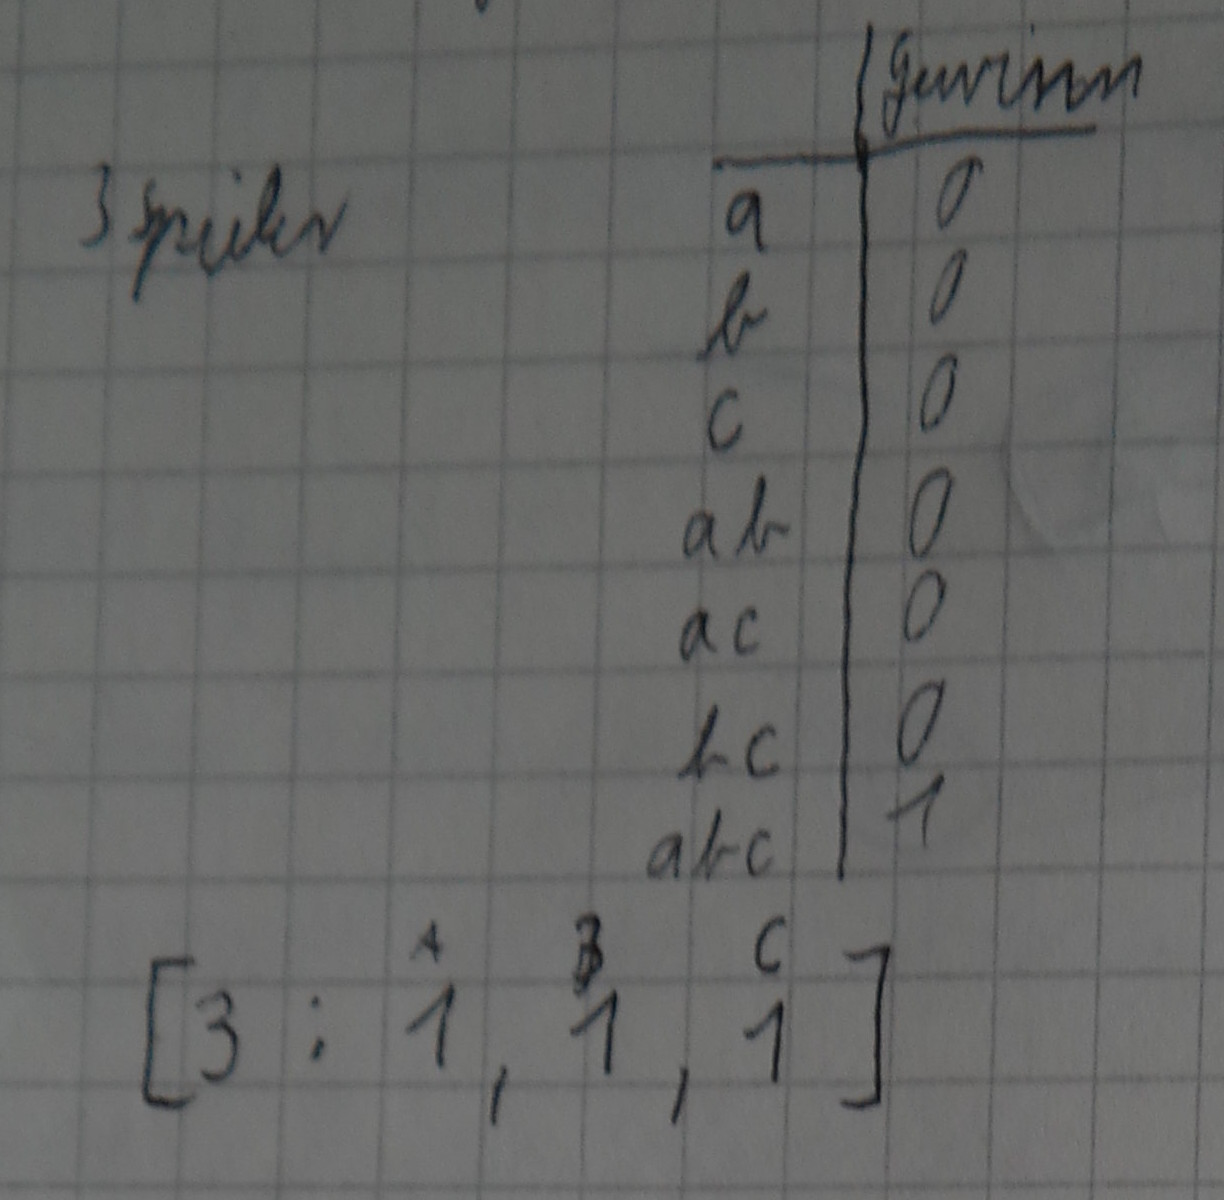
\includegraphics[scale=0.5]{aufgabeA}\\
\end{center}

b) Das dier erwirtschaftete Gewinn hier nur 1 oder 0 sein darf, müssen sich alle
        Spieler die keine Dummy-Spieler sind den Gewinn teilen. Würde ein
        Dummy-Spieler einen Teil des Gewinns erhalten, wäre die Koalition nicht mehr
        stabil. Dann würde es sich für die restlichen Spieler lohnen den Dummy-Spieler
        aus der Koalition zu entfernen um den Gewinn nur unter sich zu teilen.

\begin{center}
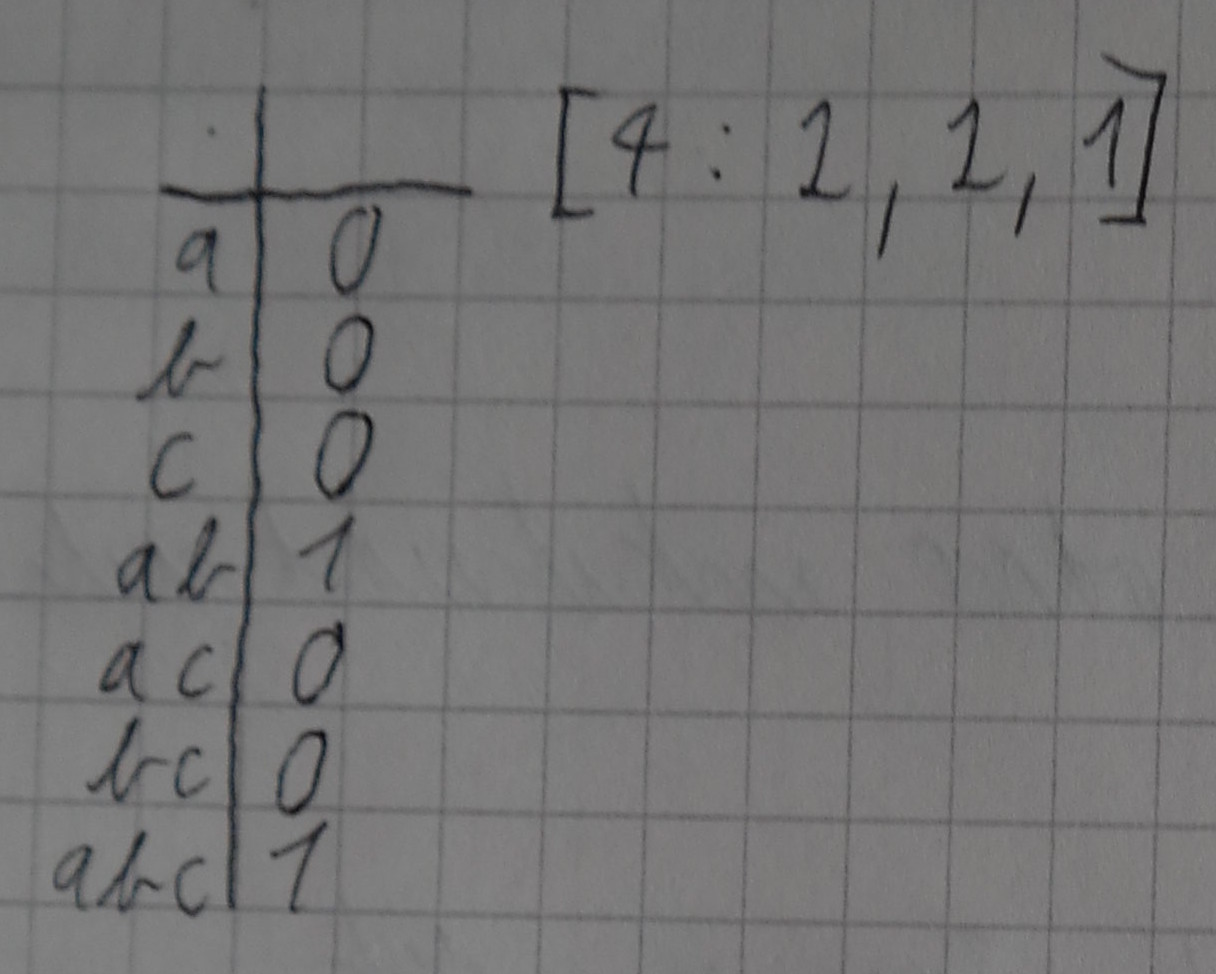
\includegraphics[scale=0.5]{aufgabeB}\\
\end{center}

c) In dem Spiel [4: 2, 2, 1] sind Spieler A und B Vetospieler, da ohne einen
        von beiden nie eine Koalition zustande kommen kann. daraus folgt, dass es
        WVG mit mehr als einem Vetospieler gibt.\\

d) Da in einem Spiel mit einem Diktator immer der Diktator den Gewinn bekommt
        und nie ein anderer Spieler ohne den Diktator, können weitere Spieler niemals
        einen Zugewinn in die Koalition einbringen. Daraus resultiert, dass dieses
        Spiel immer Superadditiv ist.

\begin{center}
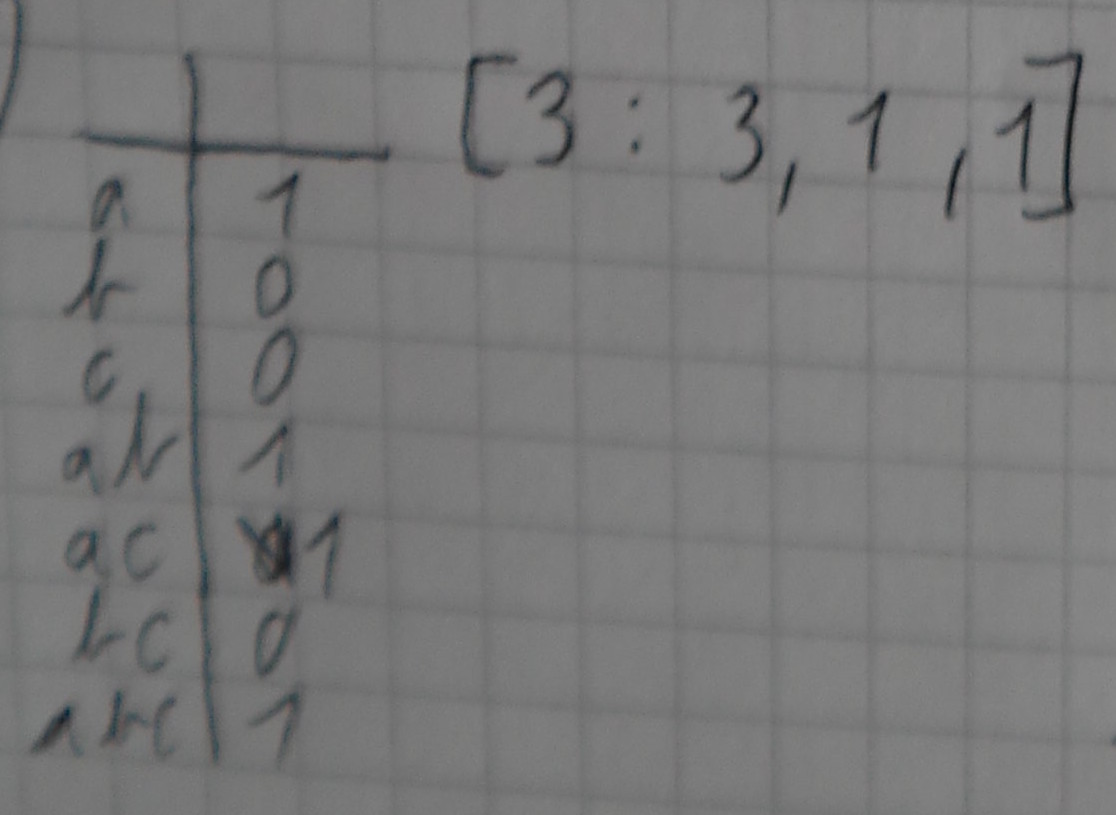
\includegraphics[scale=0.5]{aufgabeD}\\
\end{center}

e) Die Aussage stimmt nicht. In d) wurde gezeigt, dass das Spiel mit einem
        Diktator Superadditv ist. Da der Diktator der Einzige ist, der Gewinn
        erwirtschaftet, sind alle Koalitionen, an denen der Diktator beteiligt ist,
        im Core, wenn er allein den Gewinn erhält.\\

\end{document}
